\documentclass[11pt,a4paper]{article}
\usepackage[english]{babel}
\usepackage{amsfonts,amsmath,amssymb}
\usepackage{graphicx}
\usepackage{subfig} %for figures next to each other

\usepackage{hyperref} % for hyperlinks

\usepackage{listings} % for writing codes in latex
\usepackage{color}

\textheight25.5cm
\textwidth16.2cm
\voffset-2.4cm
\hoffset-1.8cm


\definecolor{dkgreen}{rgb}{0,0.6,0}
\definecolor{gray}{rgb}{0.5,0.5,0.5}
\definecolor{mauve}{rgb}{0.58,0,0.82}

\lstset{frame=tb,
  language=Python,
  aboveskip=3mm,
  belowskip=3mm,
  showstringspaces=false,
  columns=flexible,
  basicstyle={\small\ttfamily},
  numbers=none,
  numberstyle=\tiny\color{gray},
  keywordstyle=\color{blue},
  commentstyle=\color{dkgreen},
  stringstyle=\color{mauve},
  breaklines=true,
  breakatwhitespace=true,
  tabsize=3
}

\renewcommand{\familydefault}{\sfdefault}


%------------------------------------------------------------
%		ORDER of SECTIONS
%
%		Title
%		Author's name and institutional affiliation
%		Author note
%		Abstract
%		Introduction
%		...
%		References
%		Appendices and supplemental materials


\begin{document}
\title{\textbf{Spam e-mail classifiers using spambase dataset}}

\author{
	Alexander Bj\"ornsson\\
	{\tt alexanderb13@ru.is}
\and
	Sara Sabrina Zemlji\v c \\
	{\tt sara.zemljic@gmail.com}
}

\date{{\small School of Computer Science\\ Reykjavik University, Iceland}\\
\medskip
{\small \today}}
\maketitle

\begin{abstract}
We can all agree that the amount of spam we get every day by e-mail is almost limitless. The annoying spam messages are also getting more and more dangerous since they may contain viruses or other threats. Therefore it is of no surprise that spam filters have been studied quite intesively with various methods from machine learning.

We present our models for spam filtering on the dataset spambase using methods like $k$ nearest-neighbors, Na\"ive Bayes and neural networks.
\end{abstract}

\medskip
\textbf{Keywords:} e-mail, spam, false positives, $k$ nearest-neighbors ($k$NN), Na\"ive Bayes (NB), artificial neural network (ANN).
\medskip

\section{Introduction}

Cormack~\cite[p.2]{Cormack-2006} defined spam as \textit{unwanted communication intended to be delivered to an indiscriminate target, directly or indirectly, notwithstanding measures to prevent its delivery.} Very commonly people would also denote not-spam e-mails as {\em ham}.
Spam nowadays can have different purposes but it generally presents a threat for receiver so researchers have been looking for ways to prevent spam e-mails being opened but such that ham messages would not be effected by them. 
% false positives
Here it is very important to note that classifying a spam message wrongly as a ham is not as bad as classifying a ham message as a spam. So when comparing models we are mainly just interested in whether a model gives us lower values for false positives.

Let us first list a few models that have been trained for e-mail spam detection. Even though it is not really up-to-date anymore, Cormack~\cite{Cormack-2006} gives a very extensive overview of most important spam filter techniques both, hand-crafted and machine-learning ones. Among most popular are $k$NN, ANN, support vector machines (SVM), and also Bayesian methods. The latter ones have a lot of possibilities and they often depend on distribution of particular attributes in datasets. Most of the options on Na\"ive Bayesian classifiers were compared and studied in~\cite{Metsis-2006}, as well as recently in~\cite{Eberhardt-2015} and~\cite{sah-2017}, where NB was compared to SVM. ANN for spam e-mail filtering has been studied in~\cite{puniskis-2006}, ~\cite{Idris-2011} and has been compared to different other classifiers in~\cite{deepa-2010}.
%
There were also several papers focusing on feature selection and parameters optimization~\cite{lee-2010} or on content-based classification~\cite{saab-2014}. An intriguing add-on to the very extensive research on spam filters is another recent paper~\cite{asadi-2017} studying unsupervised neural network methods which were then applied on several datasets including our spambase.


%\textbf{maybe also why we decided for this dataset out of all others: the others would require way too much preprocesing with HTML and stuff like that which is not soooo relevant to this project}\\


The rest of our paper is organized as follows. In the next section we introduce our dataset and what preprocesing we performed on it. In Section~\ref{sec-models} we discuss the classifiers we trained and their performance is presented in Section~\ref{sec-evaluation}. We conclude the paper with final thoughts about the filters and present our code in the appendix.

\section{Dataset}
\label{sec-data}

The dataset we are using for this research is the {\em spambase}, a SPAM E-mail Database~\cite{spambase} donated by George Forman (gforman at nospam hpl.hp.com, 650-857-7835) from Hewlett-Packard Labs and was generated in June/July 1999. 
The spam e-mails in the collection include advertisements for products or web sites, make money fast schemes, chain letters, etc. The collection of non-spam e-mails in the database came from filed work and personal e-mails, therefore the dataset is very specific. For example words like 'george' or the code '650' are very strong indicators that an e-mail is not spam. 

There are 4601 instances out of which 1813 (about 39.4$\%$) are spam. Each instance is represented as a vector with 58 entries, so 57 + 1 columns, out of which
\begin{itemize}
  \item[--] the last one gives us the class information, it is either 1 (= spam) or 0 (= ham);
  \item[--] first 48 columns are continuous real attributes in the range $[0,100]$ of type {\tt word\_freq\_WORD} (e.g.\ {\tt word\_freq\_make}, {\tt word\_freq\_address}, {\tt word\_freq\_all}, etc.). 
  These attributes present the ration of the number of times the {\tt WORD} appears in the e-mail) over the total number of words in e-mail.  A "word" in this case is any 
string of alphanumeric characters bounded by non-alphanumeric characters or end-of-string.
  \item[--] next 6 columns are continuous real attributes in the range $[0,100]$ of type {\tt char\_freq\_CHAR} (e.g.\ {\tt char\_freq\_;}, {\tt char\_freq\_!}, {\tt char\_freq\_\$}), 
  which present the percentage of characters in the e-mail that match {\tt CHAR}.
  \item[--] last 3 attributes are continuous real in the range $[1,\ldots ]$ and are a bit special. They count occurences with capital letters. For example, {\tt capital\_run\_length\_average} counts average length of {\em uninterrupted sequences of capital letters}.
\end{itemize}

This dataset is preprocesed, which means the attributes were chosen this way to classify spam the best when they introduced the dataset in 1999. It also has no missing values. The data is not available in the raw format, so it is imposible to experiment with other attributes that could be extracted from their e-mails. Despite that this dataset was used in various studies for testing different classifiers for recognizing spam e-mails.

First we split our data into train and test sets, using $20\%$ of the data for testing our models at the end. For all calculations presented in Section~\ref{sec-models} we thus only use train part of the data. Furthermore, to ensure that we are always using the same train set we included the same {\tt random\_state} in all calculations. Our classes (spam-ham) are in about $2:3$ ratio, so we checked that the train-test split has a similar ratio of spam and ham e-mails as well. 

For some of our models we required normalized data. We assume some outliers in our data therefore we use standard score normalization (in scikit-learn this corresponds to {\tt norm='l2'} when using normalize {\tt function}). 
\bigskip

\section{Models}
\label{sec-models}

After studying the literature of spam e-mail filters, in particular what has been studied on the spambase dataset we have decided to find a spam filter classifiers for our dataset with three different methods. First we used $k$ nearest-neighbour classifier, then we studied Na\"ive Bayes methods on our dataset and finally we have built an artificial neural network classifier. In Section~\ref{sec-evaluation} we will discuss which of the models fits best for our dataset.

Let us once again mention that we are mainly interested in minimizing the false positives because we thing classifying a regular e-mail as spam is much larger sin than having one or two spam e-mails in our mailbox. Therefore we merely focus on precision rather than accuracy of our models.

\newpage
\noindent
\framebox[1.1\width]{\textbf{$k$ nearest-neighbour classifier}}

\smallskip

Our data has 57 attributes, that means we are dealing with 57-dimensional space and with "only" 4601 instances, which makes them very sparse in the space. Therefore we have decided to first reduce dimensionality of the dataset using Principle Component Analysis (PCA). In general, the more we reduce the dimensionality the better, but on the other hand using just a single component of the dataset might hide some important characteristics of data. 
\begin{figure}[ht!]
\centering
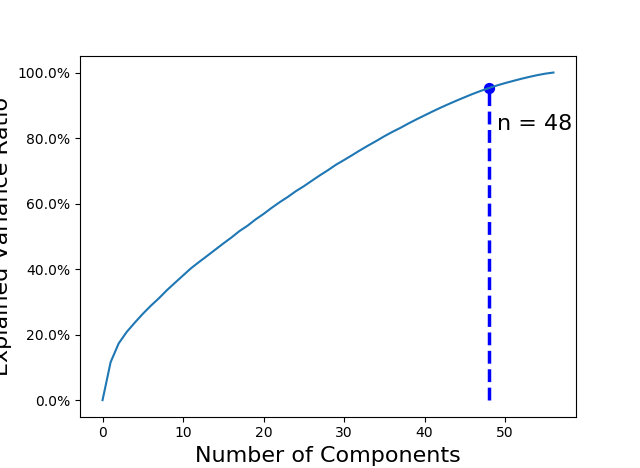
\includegraphics[scale=0.60]{n_components.png}
\caption{Variance of data represented by components in PCA}
\label{fig:n-components}
\end{figure}
First we looked at what number of components we would still have 95$\%$ of variance of our data. This gave us 48 components (see Figure~\ref{fig:n-components}), but since this is still quite high number for dimensionality for $k$NN model we decided to research which number of components would give us best results for a simple (standard\footnote{Standard is refering to default value suggested by scikit learn, which is $k=5$.}) $k$NN model. Using 10-fold cross-validation and precision we deducted that {\tt n\_components} should be 14. These results are presented in Figure~\ref{fig:hypertune_n_components} (For more details see the code in the Appendix.)
\begin{figure}[ht!]
\centering
\hspace*{-17mm}
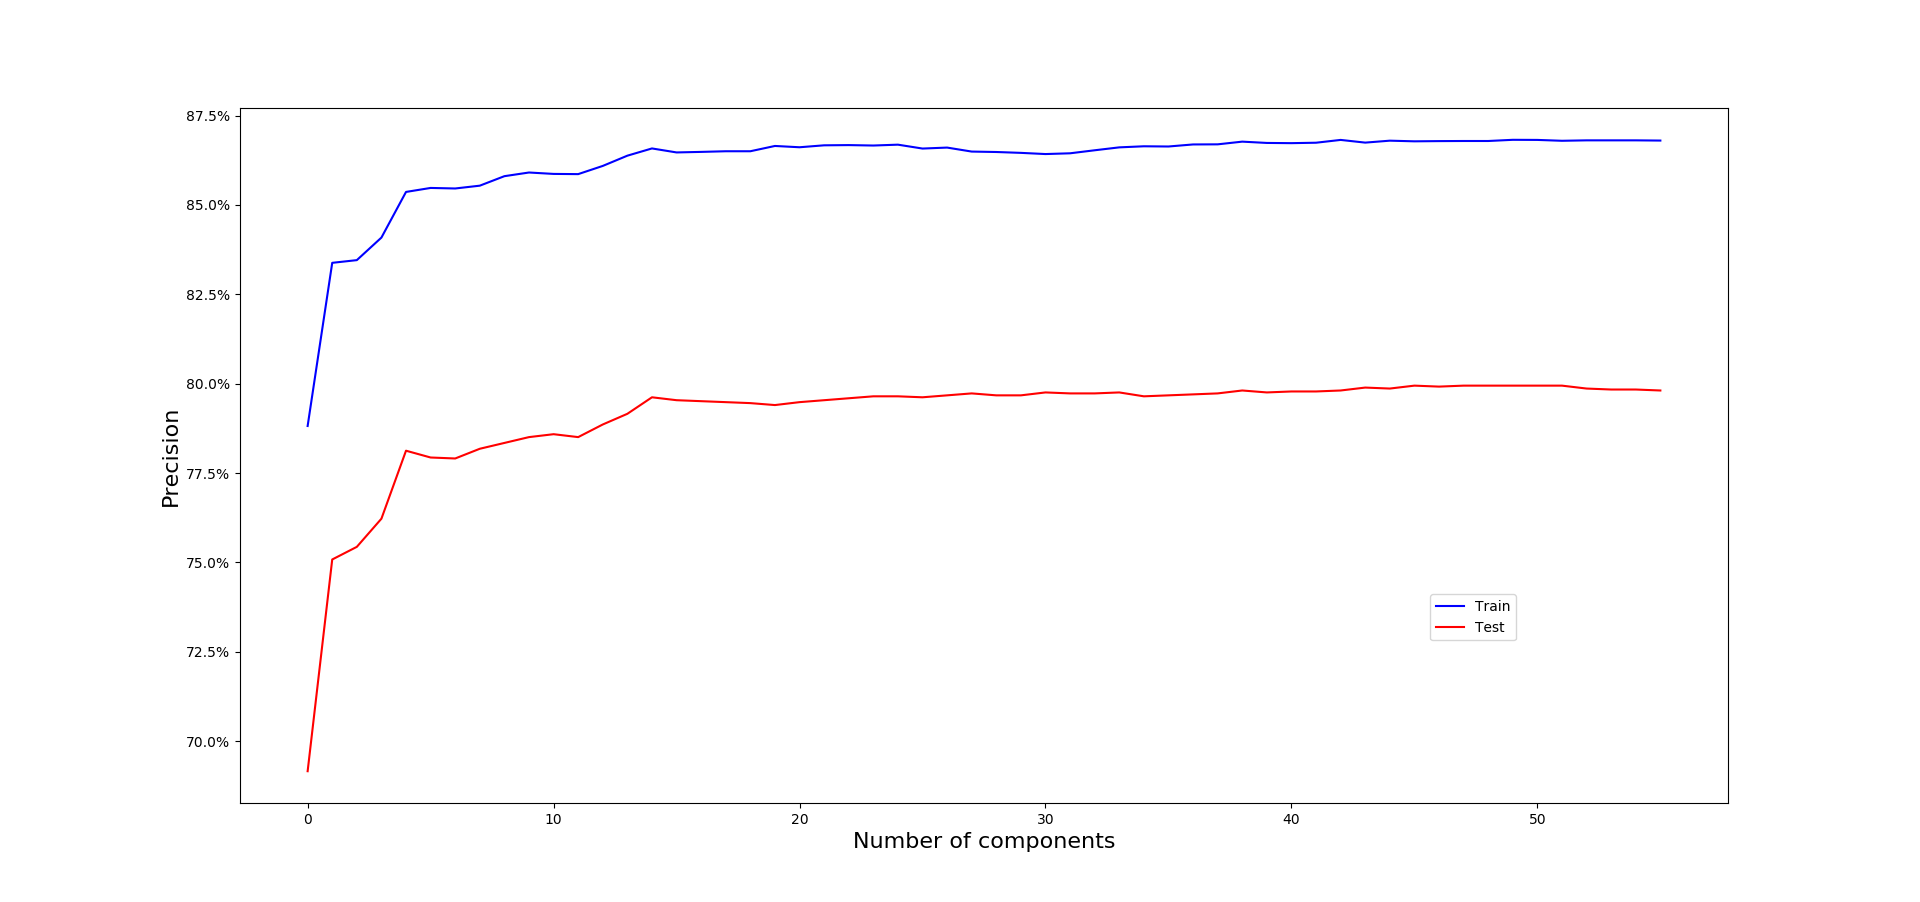
\includegraphics[scale=0.40]{hypertune_n_components_recall.png}
\caption{Precision in relation to number of components in PCA}
\label{fig:hypertune_n_components}
\end{figure}

Now that we set the number of components in PCA to 14 we can focus on $k$NN and try to find the best parameters for $k$NN for our data. To determine what number of neighbors to look at we applied yet another cross-validation: we look at precision for $k\in [1,100]$, see Figure~\ref{fig:Hypertune_kNearest}. The best precision on test data we get with $k=4$.
\begin{figure}[ht!]
\centering
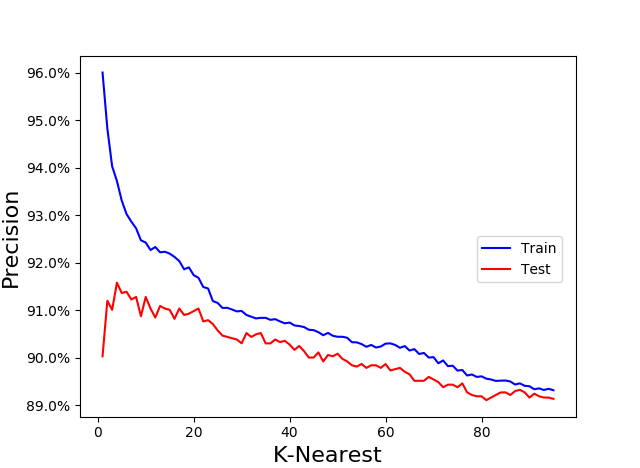
\includegraphics[scale=0.60]{Hypertune_kNearest_recall.png}
\caption{Precision in relation to number of components in PCA}
\label{fig:Hypertune_kNearest}
\end{figure}

Finally, let us check that all the preprocesing and hypertuning really gave us a better model by comparing our latest $k$NN classifier trained on 14 principal components with $k=4$ to the standard $k$NN model (that is with all of 57 attributes and $k=5$. The comparison can be found in Figure~\ref{fig:kNN_model_comparison} and we can deduct that hypertuned model clearly gives us better precision.
\begin{figure}[ht!]
\centering
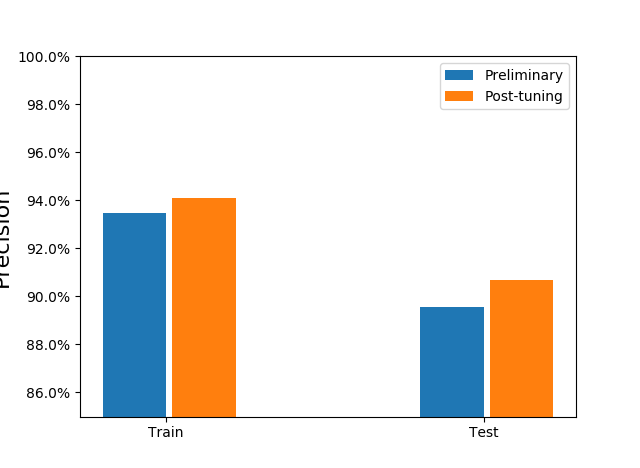
\includegraphics[scale=0.60]{kNN_model_comparison_precision.png}
\caption{Comparisson of $k$NN models}
\label{fig:kNN_model_comparison}
\end{figure}



\newpage
\noindent
\framebox[1.1\width]{\textbf{NB classifier}}

\smallskip

Using a Na\"ive Bayes method we would in general need discrete probabilities, but since we have continuous attributes in our dataset we will instead use distributions of these. There are several options for this, one of the most common ones is Gaussian Na\"ive Bayes, which assumes Gaussian (so normal) distribution of each attribute. Looking at distributions of a few attributes they all looked very similar (see Figure~\ref{fig:violinplots}) and close to multinomial distribution so we decided to use Multinomial Na\"ive Bayes instead.
\begin{figure}[ht!]
\centering
  \subfloat{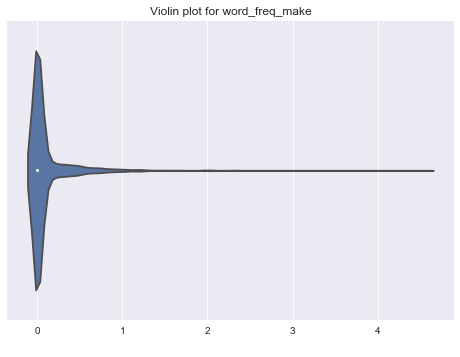
\includegraphics[scale=0.48]{violinplot0.png}}
  \hfill
  \subfloat{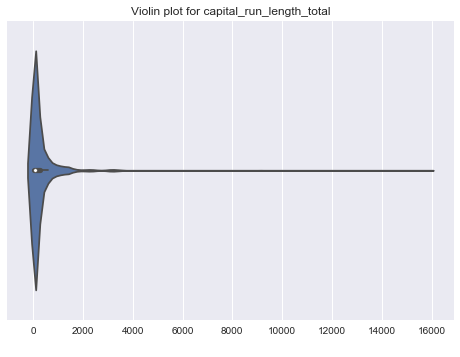
\includegraphics[scale=0.48]{violinplot56.png}}
  \caption{Distributions of attributes {\tt word\_freq\_make} and {\tt capital\_run\_length\_total}.}
\label{fig:violinplots}
\end{figure}

There are a few restrictions to multinomial distributions though. For example, our values have to be non-negative so using normalized data from the previous model does not work, but it may work if we scale those values to a non-negative range then. We have therefore tried out a few preprocesing options to see which ones would give us best results. In Figure~\ref{fig:multinomialBayes_preprocessing} for comparison of NB models built after different preprocessings. The preprocessings we test are no preprocessing, normalized data that is shifted to non-negative range, and finally normalized data that is then scaled on the interval between $[0, 1]$. 
%
\begin{figure}[ht!]
\centering
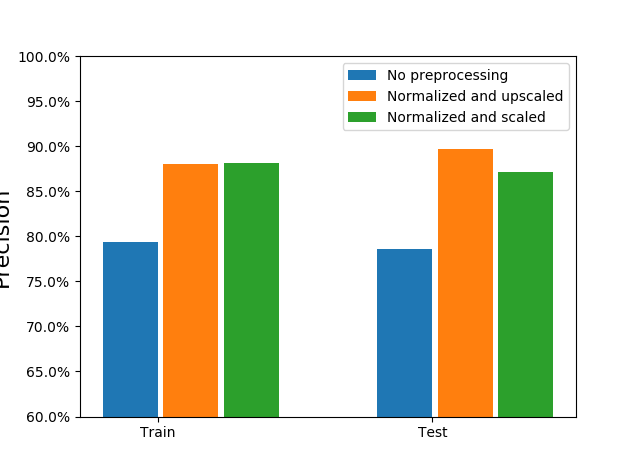
\includegraphics[scale=0.60]{mNB_preprocessing_precision.png}
\caption{Comparison of precision from different preprocessings in MultinomialNB.}
\label{fig:multinomialBayes_preprocessing}
\end{figure}
%
The best results we achieve with \textbf{** normalized dataset which is then shifted to non-negative range **}, so we use this dataset for hypertuning our model. 
\ref{fig:multinomialBayes_hypertune}.
%
\begin{figure}[ht!]
\centering
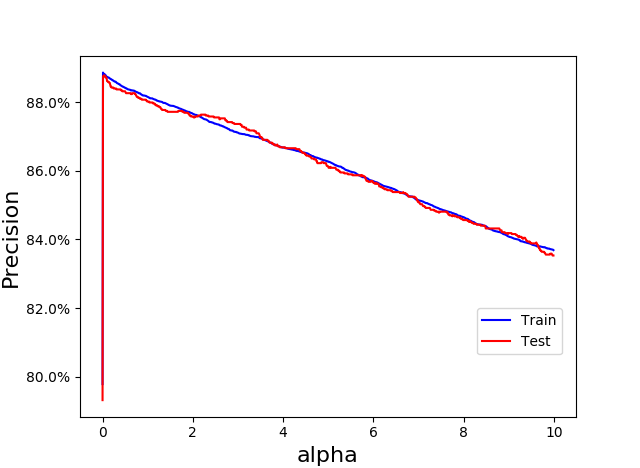
\includegraphics[scale=0.60]{hypertune_mNB_precision.png}
\caption{Hypertuning of $\alpha$ in MultinomialNB.}
\label{fig:multinomialBayes_hypertune}
\end{figure}
%
The only hypertuning we can do with MultinomialNB classifier is adjusting $\alpha$ value, which is introduced, similarly as $m$-estimate for regular NB, for handling $0$s in probabilities that we get. If any of the probabilities is $0$ we would get the whole product $=0$ and this would hide all the information of the other probabilities. 
Hypertuning using 10-fold cross-validation gives us the results presented on Figure~We figured {\em lidstone smoothing}\footnote{Lidstone smoothing means $\alpha <1$, see \cite[1.9.]{scikit} for more information.} with $\alpha$ as small as possible gives best results, so we decided to make a final NB model with $\alpha = 0.01$. 

Finally we compare the hypertuned NB model with a NB model that we would have gotten on no-preproced data with no hypertuning. We significantly increased precision both on train and test data.
\begin{figure}[ht!]
\centering
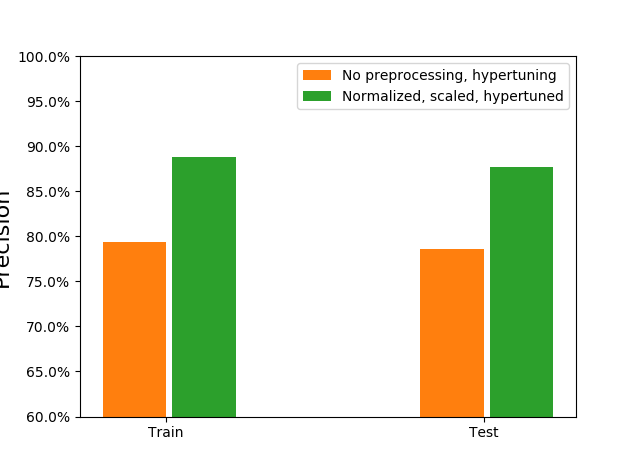
\includegraphics[scale=0.60]{mNB_model_comparison_precision.png}
\caption{Comparisson of MultinomialNB models.}
\label{fig:mNB_model_comparison_precision}
\end{figure}



\newpage
	\noindent
\framebox[1.1\width]{\textbf{ANN classifier}}

\smallskip

-- what is with ANN?


\section{Evaluation of models}
\label{sec-evaluation}

	bla bla introduction text :D


-- confusion matrix for each of them (figures)



-- precision for each of them

kNN:
Precision of the basic kNN: 0.89576547231270354
Precision of the final kNN: 0.92073832790445165

mNB:
Precision of the basic mNB: 0.78610206297502716
Precision of the final mNB: 0.87730727470141145

ANN:


-- accuracy for each of them

kNN:
Accuracy of the basic kNN: 0.895765472313
Accuracy of the final kNN: 0.920738327904

mNB:
Accuracy of the basic mNB: 0.786102062975
Accuracy of the final mNB: 0.633007600434

ANN:


\section{Conclusions}

	-- future topics: build a super model out of all three of ours




\begin{thebibliography}{99}
%!! ALPHABETICALLY!!
\begin{small}
\bibitem{Metsis-2006}
  I.\ Androutsopoulos, V.\ Metsis, G.\ Paliouras,
  Spam filtering with Naive Bayes -- Which Naive Bayes?,
  in: Proceedings of the Third Conference on Email and AntiSpam (2006).

\bibitem{asadi-2017}
  R.\ Asadi, S.\ Abdul Kareem, M.\ Asadi, S.\ Asadi, 
  An unsupervised feed forward neural network method for efficient clustering,
  The International Arab Journal of Information Technology 14(4) (2017) 436--441.

\bibitem{Cormack-2006}
  G.\ V.\ Cormack, 
  Email spam filtering: A systematic review,
  Foundation and Trends in Information Retrieval (2006) 1(4) 335--455.

\bibitem{deepa-2010}
  R.\ Deepa Lakshmi, N.\ Radha, 
  Supervised learning approach for spam classification analysis using data mining tools,
  International Journal on Computer Science and Engineering 2(9) (2010) 2783--2789.

\bibitem{Eberhardt-2015}
  J.\ Eberhardt, 
  Bayesian Spam Detection,
  Scholarly Horizons: University of Minnesota, Morris Undergraduate Journal  2(1) (2015).

\bibitem{Idris-2011}
  I.\ Idris, 
  E-mail spam classification with artificial neural network and negative selection algorithm,
  International Journal of Computer Science \& Communication Networks 1(3) (2011) 227--231.

\bibitem{lee-2010}
  S.\ M.\ Lee, D.\ S.\ Kim, J.\ H.\ Kim, J.\ S.\ Park, 
  Spam detection using feature selection and parameters optimization,
  in: Proceedings of the 2010 International Conference on Complex, Intelligent and Software Intensive Systems (CISIS) (2010).

\bibitem{spambase}
  M.\ Hopkins, E.\ Reeber, G.\ Forman, J.\ Suermondt, 
  SPAM e-mail database,
  Hewlett-Packard Labs, 1501 Page Mill Rd., Palo Alto, CA 94304,
  \url{https://archive.ics.uci.edu/ml/datasets/spambase}.

\bibitem{puniskis-2006}
  D.\ Puni\v skis, R.\ Laurutis, R.\ Dirmeikis,
  An artificial neural nets for spam e–mail recognition,
  Elektronika ir Elektrotechnika (Electronics and Electrical Engineering) 5(69) (2006) 73--76.

\bibitem{saab-2014}
  S.\ A.\ Saab, N.\ Mitri, M.\ Awad, 
  Ham or spam? A comparative study for some content-based classification Algorithms for email filtering,
  in: Proceedings of the 17th IEEE Mediterranean Electrotechnical Conference (2014).

\bibitem{sah-2017}
  U.\ K.\ Sah, N.\ Parmar, 
  An approach for malicious spam detection in email with comparison of different classifiers,
  International Research Journal of Engineering and Technology 4(8) (2017) 2238--2242.        

\bibitem{scikit}
  {\url http://scikit-learn.org/stable/index.html}
\end{small}
\end{thebibliography}

\newpage
\section*{Appendix: code}
%STRUCTURE THE CODE into smaller segments, we will only have main training parts here (no prints, no confusion matrices codes etc). Only main models and their preprocesing, for results we will just analyze them with words
	\begin{lstlisting}
import numpy as np
import pandas as pd
import matplotlib.pyplot as plt

from sklearn.neighbors import KNeighborsClassifier
from  sklearn.model_selection  import  train_test_split
from sklearn.naive_bayes import MultinomialNB
from sklearn.decomposition import PCA
from sklearn.discriminant_analysis import LinearDiscriminantAnalysis
from matplotlib.ticker import FuncFormatter
from sklearn.model_selection import KFold
from  sklearn.model_selection  import  train_test_split
from sklearn.preprocessing import Normalizer
from sklearn.metrics import precision_score

from sklearn.metrics import confusion_matrix

"""
loading and preprocesing the data
"""

file = open("spambase.data")
data = np.loadtxt(file,delimiter=",")

X = data[:, 0:57]
y = data[:, 57]

dataframe = pd.DataFrame(data=X)

#apply normalization function to every attribute
dataframe_norm = dataframe.apply(lambda x: (x - np.mean(x)) / np.std(x))

"""
kNN model
"""
# explained_variance_ratio_ for n_components
EVC = []
for attribute in dataframe_norm:
    pca = PCA(n_components=attribute)
    pca.fit(dataframe_norm)
    EVC.append(pca.explained_variance_ratio_.sum())

# n_components hyperparameter tuning using KFold cross-validation
splits = 10
kf = KFold(n_splits = splits)
n_components_kFold_train = np.zeros(n_attributes-1)
n_components_kFold_test = np.zeros(n_attributes-1)
kFold_train_precision = np.zeros(n_attributes-1)
kFold_test_precision = np.zeros(n_attributes-1)
for i in range(1, n_attributes):
    X = pca(i, dataframe)
    # Using the same random_state ensures we do not contaminate our training data with our test data
    X_train ,  X_test ,  y_train ,  y_test = train_test_split(X,  y,  test_size=0.20 ,  random_state=42)
    for cv_train_index, cv_test_index in kf.split(X_train):
        X_cv_train = [X_train_1[i] for i in cv_train_index]
        y_cv_train = [y_train_1[i] for i in cv_train_index]
        X_cv_test = [X_train_1[i] for i in cv_test_index]
        y_cv_test = [y_train_1[i] for i in cv_test_index]
        # k = 5 by defult
        kNN = KNeighborsClassifier()
        kNN.fit(X_cv_train, y_cv_train) 
        kFold_train_precision[i-1] += precision_score(y_cv_train, kNN.predict(X_cv_train), average = 'micro') / splits
        kFold_test_precision[i-1]  += precision_score(y_cv_test, kNN.predict(X_cv_test), average = 'micro') / splits

# n_neighbors cross-validation
n_components = 14 
X = pca(n_components, dataframe_norm)
X_train ,  X_test ,  y_train ,  y_test = train_test_split(X,  y,  test_size=0.20 ,  random_state=42)

k_tests = list(range(1, 100))
k_precision_train = np.zeros(len(k_tests))
k_precision_test = np.zeros(len(k_tests))

kf = KFold(n_splits = splits)
for cv_train_index, cv_test_index in kf.split(X_train):
        X_cv_train = [X_train[i] for i in cv_train_index]
        y_cv_train = [y_train[i] for i in cv_train_index]
        X_cv_test = [X_train[i] for i in cv_test_index]
        y_cv_test = [y_train[i] for i in cv_test_index]
        i=0
        for test in k_tests:
            kNN = KNeighborsClassifier(n_neighbors = test)
            kNN.fit(X_cv_train, y_cv_train) 
             k_precision_train [i-1] += precision_score(y_cv_train, kNN.predict(X_cv_train), average = 'micro') / splits
            k_precision_test [i-1]  += precision_score(y_cv_test, kNN.predict(X_cv_test), average = 'micro') / splits
            i += 1

X_train ,  X_test ,  y_train ,  y_test = train_test_split(dataframe_norm,  y, test_size=0.20 , random_state=42)

kNN = KNeighborsClassifier(n_neighbors = k)
kNN.fit(X_train, y_train)

kNN_precision_train_pre = precision_score(y_train, kNN.predict(X_train), average = 'micro')
kNN_precision_test_pre = precision_score(y_test, kNN.predict(X_test), average = 'micro')

k = 4 
X = pca(n_components, dataframe_norm)
X_train, X_test, y_train, y_test = train_test_split(X, y, test_size=0.20 , random_state=42)

kNN_precision_train_post = precision_score(y_train, kNN.predict(X_train), average = 'micro')
kNN_precision_test_post = precision_score(y_test, kNN.predict(X_test), average = 'micro')



kNN_precision_train_post = precision_score(y_train, kNN.predict(X_train), average = 'micro')
precision_test_post = precision_score(y_test, kNN.predict(X_test), average = 'micro')


"""
NB model
"""

# Different preprocessings
dataframe = pd.DataFrame(data=X)
dataframe_norm = dataframe.apply(lambda x: (x - np.mean(x)) / np.std(x))
min_max_scaler = preprocessing.MinMaxScaler()
dataframe_norm_scaled = min_max_scaler.fit_transform(dataframe_norm)
dataframe_norm_upscaled = dataframe_norm.apply(lambda x: (x + abs(min(x))))

# No preprocessing of the data
X_train ,  X_test ,  y_train ,  y_test = train_test_split(dataframe,  y,  test_size=0.20 ,  random_state=42)
mNB = GaussianNB()
mNB.fit(X_train, y_train)
precision_train = precision_score(y_train, mNB.predict(X_train), average = 'micro')
precision_test = precision_score(y_test, mNB.predict(X_test), average = 'micro')

# Upscaled normalized data with no negative attributes
X_train ,  X_test ,  y_train ,  y_test = train_test_split(dataframe_norm_upscaled,  y,  test_size=0.20 ,  random_state=42)
mNB_upscaled = GaussianNB()
mNB_upscaled.fit(X_train, y_train)
norm_upscaled_precision_train = precision_score(y_train, mNB_upscaled.predict(X_train), average = 'micro')
norm_upscaled_precision_test = precision_score(y_test, mNB_upscaled.predict(X_test), average = 'micro')


# Scaled normalized data 
X_train ,  X_test ,  y_train ,  y_test = train_test_split(dataframe_norm_scaled,  y,  test_size=0.20 ,  random_state=42)
mNB_scaled = GaussianNB()
mNB_scaled.fit(X_train, y_train)
norm_scaled_precision_train = precision_score(y_train, mNB_scaled.predict(X_train), average = 'micro')
norm_scaled_precision_test = precision_score(y_test, mNB_scaled.predict(X_test), average = 'micro')


# kFold cross-validation for alpha
splits = 10
kf = KFold(n_splits = splits)

X_train ,  X_test ,  y_train ,  y_test = train_test_split(dataframe_norm_scaled,  y,  test_size=0.20 ,  random_state=42)

alpha_tests = np.arange(0, 10.0, 0.01)
alpha_cv_train = np.zeros(len(alpha_tests))
alpha_cv_test = np.zeros(len(alpha_tests))
for cv_train_index, cv_test_index in kf.split(X_train):
    X_cv_train = [X_train[i] for i in cv_train_index]
    y_cv_train = [y_train[i] for i in cv_train_index]
    X_cv_test = [X_train[i] for i in cv_test_index]
    y_cv_test = [y_train[i] for i in cv_test_index]
    i = 0
    for test in alpha_tests:
        mNB_cv = MultinomialNB(alpha=test)
        mNB_cv.fit(X_cv_train, y_cv_train)
        alpha_cv_train[i] += precision_score(y_cv_train, mNB_cv.predict(X_cv_train), average = 'micro') / splits
        alpha_cv_test[i]  += precision_score(y_cv_test, mNB_cv.predict(X_cv_test), average = 'micro') / splits
        i += 1

\end{lstlisting}


\end{document}

%%%%%%%%%%%%%%%%%%%%

\begin{lstlisting}
\end{lstlisting}

\end{itemize}




